
%%%%%%%%%%%%%%%%%%%%%%%%%%%%%%%%%%%%%%%%%%%%%%%%%%%%%%%%%%%%%%%%%%%%%%%%%%%%%%%%%%%%%%%%%%%%%%%%%%%%%%%%%%%%
% Author: Omar Portillo
%%%%%%%%%%%%%%%%%%%%%%%%%%%%%%%%%%%%%%%%%%%%%%%%%%%%%%%%%%%%%%%%%%%%%%%%%%%%%%%%%%%%%%%%%%%%%%%%%%%%%%%%%%%%

%Abstract: 0.5
%Intro: 2
%Bg: 2
%Approach/Architecture: 3
%Experiments/Results: 5
%Related Work: 1
%Conclusions: 0.5
%References:  1

%%%%%%%%%%%%%%%%%%%%%%%%%%%%%%%%%%%%%%%%%%%%%%%%%%%%%%%%%%%%%%%%%%%%%%%%%%%%%%%%%%%%%%%%%%%%%%%%%%%%%%%%%%%%
% Defining document class + packages to be used
%%%%%%%%%%%%%%%%%%%%%%%%%%%%%%%%%%%%%%%%%%%%%%%%%%%%%%%%%%%%%%%%%%%%%%%%%%%%%%%%%%%%%%%%%%%%%%%%%%%%%%%%%%%%

\documentclass[runningheads,a4paper]{llncs}

\usepackage{amssymb}
\setcounter{tocdepth}{3}
\usepackage{graphicx}
\usepackage{epstopdf}
\usepackage[linesnumbered,ruled,vlined]{algorithm2e}

\usepackage{url}
\newcommand{\keywords}[1]{\par\addvspace\baselineskip
\noindent\keywordname\enspace\ignorespaces#1}

\begin{document}

%%%%%%%%%%%%%%%%%%%%%%%%%%%%%%%%%%%%%%%%%%%%%%%%%%%%%%%%%%%%%%%%%%%%%%%%%%%%%%%%%%%%%%%%%%%%%%%%%%%%%%%%%%%%
% TITLE + AUTHORS' INFORMATION
%%%%%%%%%%%%%%%%%%%%%%%%%%%%%%%%%%%%%%%%%%%%%%%%%%%%%%%%%%%%%%%%%%%%%%%%%%%%%%%%%%%%%%%%%%%%%%%%%%%%%%%%%%%%

\mainmatter  % start of an individual contribution

% first the title is needed
\title{An automation approach to apply idle-time analysis efficiently in a
performance testing scenario}

% a short form should be given in case it is too long for the running head
\titlerunning{Pending to define title}

% the name(s) of the author(s) follow(s) next
%
% NB: Chinese authors should write their first names(s) in front of
% their surnames. This ensures that the names appear correctly in
% the running heads and the author index.
%
\author{Andres-Omar Portillo-Dominguez\inst{1}\and Miao Wang\inst{1}\and Philip
Perry\inst{1} \and\\
John Murphy\inst{1} \and Nick Mitchell\inst{2}\and Peter F. Sweeney\inst{2}}

\authorrunning{Pending to define title}
% (feature abused for this document to repeat the title also on left hand pages)

\urldef{\mailucdconnect}\path|andres.portillo-dominguez@ucdconnect.ie,|
\urldef{\mailucd}\path|{philip.perry,miao.wang,j.murphy}@ucd.ie,|
\urldef{\mailibm}\path|{nickm,pfs}@us.ibm.com|

% the affiliations are given next; don't give your e-mail address
% unless you accept that it will be published
\institute{Lero - The Irish Software Engineering Research Centre, Performance\\
Engineering Laboratory, UCD School of Computer Science and Informatics,
University College Dublin, Ireland\\
\mailucdconnect\\
\mailucd\\
%\url{http://www.ucd.ie/}
\and
IBM T.J. Watson Research Center,\\
Yorktown Heights, New York, USA\\
\mailibm}%\\
%\url{http://www.ibm.com/}


\toctitle{Lecture Notes in Computer Science}
\tocauthor{Authors' Instructions}
\maketitle

%%%%%%%%%%%%%%%%%%%%%%%%%%%%%%%%%%%%%%%%%%%%%%%%%%%%%%%%%%%%%%%%%%%%%%%%%%%%%%%%%%%%%%%%%%%%%%%%%%%%%%%%%%%%
% Abstract 
%%%%%%%%%%%%%%%%%%%%%%%%%%%%%%%%%%%%%%%%%%%%%%%%%%%%%%%%%%%%%%%%%%%%%%%%%%%%%%%%%%%%%%%%%%%%%%%%%%%%%%%%%%%%

\begin{abstract}
Performance testing in highly distributed environments is a very challenging
task. Specifically, the identification of performance issues and
the diagnosis of their root causes are time-consuming and complex tasks which
heavily rely on the expertise of the engineers. As those activities commonly
require the usage of multiple tools, the required technical knowledge is even
higher. WAIT is a tool that has been successful, under the right conditions, to
reduce the dependency to the expert knowledge to simplify the identification of
performance issues and their root causes. However, it has some usability
limitations that prevent its efficient usage in performance testing. This paper
presents an light-weight approach to address those limitations and automate the 
usage of WAIT to make it useful in the performance testing domain.

This work used a 3-phase experiment to validate the approach in terms
of overhead costs, time savings and overall usefulness in the
analysis of performance issues, work that involved a case-study with two
real-life applications. The current results have proven the feasibility of the
proposed approach by achieving a good decrement in the time invested to do performance
analysis with only a low level of overhead.
\keywords{Performance testing, automation, performance analysis, idle-time
analysis}
\end{abstract}


%%%%%%%%%%%%%%%%%%%%%%%%%%%%%%%%%%%%%%%%%%%%%%%%%%%%%%%%%%%%%%%%%%%%%%%%%%%%%%%%%%%%%%%%%%%%%%%%%%%%%%%%%%%%
% Introduction
%%%%%%%%%%%%%%%%%%%%%%%%%%%%%%%%%%%%%%%%%%%%%%%%%%%%%%%%%%%%%%%%%%%%%%%%%%%%%%%%%%%%%%%%%%%%%%%%%%%%%%%%%%%%


\section{Introduction}

Nowadays quality is a key element of any software development process because it
plays a major role in the successful adoption of any software product. Moreover,
quality has a direct impact in the total cost of ownership of the software. For
example, a 2008 Quality Assurance study \cite{CapersJones1} identified that achieving 
high software quality usually generates cost savings of around 40\%: While
average software costs per function point (FP) are close to \$1,000 USD in each
of the development and maintenance phases, these costs are reduced to only \$700
USD and \$500 USD, respectively, when the software quality is above the average. 
This scenario shows the relevance of investment in quality and how it is the
right strategy to follow.

As one of the eight dimensions of quality
\footnote{http://lssacademy.com/2008/05/28/8-dimensions-of-quality/}, software
performance is a critical non-functional characteristic which is concerned
with the capacity and timeliness of the software. Furthermore it is an accepted
fact in the industry that performance is a major concern of any software
project, especially in enterprise-level applications, as performance issues
might not only affect the users’ experience, but also have a considerable financial impact. 
However it is not uncommon that performance issues materialize into serious
problems (i.e. schedule delays, cost overruns, outages on production
environments, or even cancellation of projects) in a significant percentage of
software projects. For example, a 2007 survey applied to information technology
executives \cite{Compuware1} identified that 50\% of the interviewed people had
faced performance problems with at least 20\% of their deployed applications.

In general terms, the pervasive nature of performance makes it difficult to
test it and understand the factors behind it, as performance is practically
affected by every single aspect of the design, code, and execution environment of an application.
Besides the latest trends in the information technology world (such as Service Oriented
Architecture and Cloud Computing) have augmented the complexity of the
applications further complicating the activities related to performance testing,
tuning and monitoring. Additionally, as any other software engineering activity,
these activities are usually constrained by tight project schedules and budgets.

Under the above conditions, it is not surprising that doing good performance
testing is a very complex and time-consuming task. A special challenge, documented by 
multiple authors such as \cite{Woodside2007,trevor1,Angelopoulos2012}, is the
fact that the current performance techniques and tools heavily rely on the expert knowledge of the
users to understand and analyze their output. Moreover it is common that
multiple tools are required to assess and diagnose different performance
problems, especially in highly distributed environments. For example, in
enterprise-level Java applications garbage collection logs, thread dumps, 
thread usage statistics, heap dumps, CPU utilization, JVM memory usage, 
JDBC pool status and server response time are only some of the resources a
tester can use to understand how an application is performing. It consequently
increases the technical skill set required to efficiently use such tools, which
is usually held by only a small number of experts within an organization.
This situation could potentially lead to create bottlenecks in those specific
activities that could only be carried out by these limited experts, hence
impacting the overall productivity of large testing teams where commonly the
expertise is not evenly distributed.

In addition to the previous challenges, lightweight instrumentation and
automation are old goals that continue to demand attention in the performance
testing area. In general, the overhead generated by any technique or tool
should be low in order to minimize the impact their usage might have in the
tested environment in terms of response time and throughput, otherwise it would not be
suitable to be used for performance testing. Similarly, if the techniques and
tools require a heavy human effort to be used effectively, this situation might limit 
their applicability by making them too complex to apply or error prone. As
documented by the authors of \cite{Shahamiri1}, here automation could play a key
role to encourage the adoption of the technique, as this strategy has been
successfully applied to decrease the time and costs required to perform
testing activities.

To ensure that our research work is helpful for solving real-life problems for
software industries, we have also carried out regular meetings with the IBM
System Verification Test (SVT) to discuss the challenges that they experience in
their day-to-day testing activities. The received feedback is similar in terms
that there is a real need to develop tools that can produce information which is
consumable by both domain and non-domain experts, hence helping to improvement the 
performance of the testing teams by allowing a wider number of testers to carry out 
complex system analysis in less time.

In summary, the detection of performance related issues and the identification
of their root causes have become very challenging and time consuming tasks,
especially in highly distributed environments, usually requiring not only the
usage of multiple tools to do performance triage but also heavily relying on
the expertise of the people involved on those tasks.

WAIT \footnote{http://wait.ibm.com} (an expert system that performs idle-time
analysis in Java environments based mostly in javacores) has proven successful
in simplifying the detection of performance related issues and their root causes 
in Java environments \cite{Altman2010,Wu1}. Moreover, the main strengths of WAIT
makes it an attractive candidate to the performance testing domain, as it has minimal 
impact in the monitored environment and the obtained testing results: On one
hand, WAIT uses a very light-weight monitoring approach which does not require 
any instrumentation or changes to the monitored environment. On the other hand,
WAIT also has very low overhead.

Despite its strengths, WAIT has certain usability limitations that prevent its
effective usage in the performance testing domain: The overall data collection
process needs to be done manually which makes it very time-consuming and
error-prone to use, especially in a highly distributed environment where there
would be multiple nodes to monitor and coordinate simultaneously, especially
if the data needs to be refreshed periodically during the test execution in
order to have an incremental view of the results. This last scenario is highly
desirable in long runs (i.e. 5 days or more), where the testers cannot have the
luxury of waiting until the end of the test to know if any performance issues
exist. 

Even though the above limitations might be manageable in small testing
environments or test runs (i.e. a few hours duration), they prevent WAIT to be
effectively use in bigger testing environments, as the time and effort
required to synchronize WAIT execution would overcome the possible benefits of
its usage, especially considering that this process would be highly error-prone.
As the highly distributed environments are precisely the scenarios where WAIT's
performance analysis capabilities would be more valuable to simplify the testing 
activities of identification and expedite the diagnosis of performance issues,
these usage limitations should be addressed. 

This paper proposes a lightweight automated approach that addresses the above
limitations in order to use WAIT effectively in the performance testing domain, 
while keeping WAIT's strengths of low overhead and minimal intrusion. This work
was achieved through a 3-phase experiment: The first two phases were concentrated 
in evaluating the overhead of the approach, as it was critical that the overhead remained low to avoid
compromising the performance of the tested environment. On the contrary, the third 
phase concentrated in assessing the accuracy of WAIT's results and the productivity 
improvements that it could bring to the performance testing process. 

The results of this work have provided evidence regarding the feasibility of the
proposed approach [PENDING: low overhead, easy identification of issues].

The main contribution of this paper is a lightweight approach to automate the data 
gathering and execution of WAIT in sync with a performance test loader in
order to make WAIT usable in the performance testing domain. Moreover the
approach has a low overhead and could be easily adaptable to work with other
performance analysis tools that rely on similar data sources.

The rest of this paper is structured as follows: Section 2 discusses the
background. Section 3 shows the related work. Section 4 describes the proposed
approach, including details of design and implementation. Section 5 describes
the experimental setup and methodology, while Section 6 explores the
experimental results. Finally Section 7 presents the conclusions and future
work. [PENDING to adjust to reflect the final structure]


%%%%%%%%%%%%%%%%%%%%%%%%%%%%%%%%%%%%%%%%%%%%%%%%%%%%%%%%%%%%%%%%%%%%%%%%%%%%%%%%%%%%%%%%%%%%%%%%%%%%%%%%%%%%
% Background
%%%%%%%%%%%%%%%%%%%%%%%%%%%%%%%%%%%%%%%%%%%%%%%%%%%%%%%%%%%%%%%%%%%%%%%%%%%%%%%%%%%%%%%%%%%%%%%%%%%%%%%%%%%%

\section{Background}

WAIT is a tool to do performance triage which offers a high-level view of
the whole system as well as the main performance inhibitors that exist on the
system. WAIT is based on the idle-time analysis methodology \cite{Altman2010}
which pursues to infer performance behaviors and problems based on non-intrusive sampling mechanisms
available by default in at the Operating System level (i.e. the ``ps'' or
``vmstat'' commands in a Unix/Linux environment) and the Java Virtual Machine
(in the form of javacores
\footnote{http://www-01.ibm.com/support/docview.wss?uid=swg27017906\&aid=1}
, which are a diagnostic feature available in Java to get quick snapshot of the
JVM status, including information such as threads, locks, monitors,
classloaders, classes and memory usage). The fact that WAIT uses these data
sources makes it non-disruptive to the monitored environments, as no special flags, 
service restart or instrumentations are required to use it. As WAIT also
requires infrequent samples to perform a diagnosis (at most every 30 seconds,
even though the sampling rate could be adjusted), it is low-overhead.

From a usability perspective, WAIT is simple: A user only needs to
collect as much data as desired (either manually or using gathering scripts
that are available for the most common operating systems), and then upload the
data to a central repository (throughout a web interface) to obtain a web 
report with the findings. Internally, WAIT uses a centralized knowledge base,
which is an engine built on top of a set of expert rules that have been the result of a 
deep analysis and sophisticated understanding of the Java main frameworks and
libraries. This centralization schema offer the additional benefit that
the rules and knowledge base can continue growing and evolving over time.

%%%%%%%%%%%%%%%%%%%%%%%%%%%%%%%%%%%%%%%%%%%%%%%%%%%%%%%%%%%%%%%%%%%%%%%%%%%%%%%%%%%%%%%%%%%%%%%%%%%%%%%%%%%%
% Related Work
%%%%%%%%%%%%%%%%%%%%%%%%%%%%%%%%%%%%%%%%%%%%%%%%%%%%%%%%%%%%%%%%%%%%%%%%%%%%%%%%%%%%%%%%%%%%%%%%%%%%%%%%%%%%

\section{Related Work}

[PENDING to review/merge my literature review notes]


%%%%%%%%%%%%%%%%%%%%%%%%%%%%%%%%%%%%%%%%%%%%%%%%%%%%%%%%%%%%%%%%%%%%%%%%%%%%%%%%%%%%%%%%%%%%%%%%%%%%%%%%%%%%
% Problem Definition
%%%%%%%%%%%%%%%%%%%%%%%%%%%%%%%%%%%%%%%%%%%%%%%%%%%%%%%%%%%%%%%%%%%%%%%%%%%%%%%%%%%%%%%%%%%%%%%%%%%%%%%%%%%%

\section{Problem Definition}

While doing performance testing in highly distributed environments, the
identification of performance problems and the diagnosis of their root causes are very complex and time-consuming
activities, which tend to rely on the expertise of the involved engineers.

Due to its strengths, WAIT is a promising candidate that can help to improve the
above scenario by reducing the expert knowledge and time required to do good
performance analysis. However, WAIT currently has some usability limitations
that prevent its effective usage in the performance testing domain. More
specifically, the effort required to do manual data collection to feed WAIT is
practically lineal with respect of the number of nodes that need to be monitored
and the frequency with which the data needs to be refreshed. For example,
assuming an scenario of a relatively small distributed environment composed
of 10 application nodes during a 24-hour test run and with a desired refresh
frequency of 60 minutes, it would mean that the tester would need to coordinate 
24 data collection and upload cycles per node (for a total of 240
cycles in this example), making sure to do them as far as possible in order to
minimize the time gaps between the end of a data collection cycle and the
start of the next one. Additionally, the tester should also synchronize this
process with the performance testing duration. In order to get the most value
out of WAIT, the tester should also review the reports he would get after every 
upload in order to see if any major issue has been detected. As it can be easily inferred from
the above scenario, the current costs of using WAIT under the above conditions
overcome the possible benefits of using it, especially after adding the high
possibility of a human error which might compromise the obtained results.

The objective of this paper is to address the usability limitations of WAIT to
be used effectively in the performance testing domain. In order to do it, the
following research questions have been formulated:
\\Q1. How can the usage of WAIT be automated to minimize the effort
required to use it in sync with the performance testing?
\\Q2. How can the overhead be kept low during the whole performance test
execution to avoid compromising the results? 
\\Q3. What benefits in productivity can a tester achieve if the previous
questions are answered?

The following sections show in details how they have been answered by our
approach and validated through a series of experiments.

%%%%%%%%%%%%%%%%%%%%%%%%%%%%%%%%%%%%%%%%%%%%%%%%%%%%%%%%%%%%%%%%%%%%%%%%%%%%%%%%%%%%%%%%%%%%%%%%%%%%%%%%%%%%
% Proposed Approach
%%%%%%%%%%%%%%%%%%%%%%%%%%%%%%%%%%%%%%%%%%%%%%%%%%%%%%%%%%%%%%%%%%%%%%%%%%%%%%%%%%%%%%%%%%%%%%%%%%%%%%%%%%%%

\section{Proposed Approach and Implementation}

This section presents the details of the proposed approach, its architecture
and the prototype that has been developed to validate it.

Our approach is depicted in the Algorithm~\ref{Proposed_Approach} and requires
a few inputs: First of all, the list of nodes (either IP addresses or names that
can be resolved by a Domain Name System) that will be monitored (which
will usually be all the nodes that composed the system that will be tested); a
\emph{Sampling Interval} to control how often the samples will be collected
from the data sources; a \emph{Time Threshold} which indicates what is the
maximum time that could pass without refreshing the results; a \emph{Hard Disk
Threshold} which indicates what is the maximum space that can be used in each
node to store collected data; and finally a \emph{Backup} flag that indicates if
(and where) the collected data should be backed up before any clean process could start.

After having this information the process starts by getting a new \emph{RunId},
value that will uniquely identify the test run and its results. This value is
then propagated to all the nodes. On each node, the \emph{Hard Disk Usage} is
initialized as well as the \emph{Next Time Threshold}. Then each nodes starts
executing the following iterative steps until the performance test finishes:
First a new set of data samples is collected (composed of machine and process
utilization plus a Javacore from every JVM running in the node). Once the data 
has been collected, it is assessed if any of the two thresholds has been reached 
(either the \emph{Hard Disk Usage} has exceeded the \emph{Hard Disk
Threshold} or the \emph{Next Time Threshold} has been reached). If any of this
conditions has occurred, a new upload process occurs where all the collected
data is transmitted to the central repository of WAIT (marking it with the
\emph{RunId} so that all uploads are related to the same performance test).
Moreover, if a \emph{Backup} was indicated the data is also copied to the
backup destination before it is deleted. Then a reference to the updated results
report is obtained and the \emph{Next Time Threshold} is calculated. Finally,
the logic awaits the configured \emph{Sampling Interval} and then a new iteration starts.

Once the performance test finishes, a final upload round (and backup if
configured) is done to upload any remnant collected data. When completed this
data is also cleared and the \textbf{final performance results report} is
obtained.

\begin{algorithm}
\caption{Proposed Approach}
\label{Proposed_Approach}
\DontPrintSemicolon
\KwIn{ A finite set $A=\{a_1, a_2, \ldots, a_n\}$ of application nodes, 
Sampling Interval \emph{Sint}, Time Threshold \emph{tThres}, Hard Disk Threshold
\emph{hdThres}, Backup Flag \emph{bFlag}. 
If \emph{bFlag} = true, Backup path \emph{bPath}.}
\KwOut{Consolidated Performance Analysis Results for all Nodes}
\tcp*[h]{Initialization}\;
$rundId \gets $new RunId\;
share $rundId$ \hspace{2 mm} with all nodes\;
\For{$i \gets 1$ \textbf{to} $n$} {	
	$hdUsage \gets 0$\;
	$nextTimeThreshold \gets $current time from the Operating System + $tThres$\;
			
    \tcp*[h]{Main Process}\;
	\While{performance testing is executing}{
		\tcp*[h]{Data gathering}\;
		Collect new set of samples (process and machine utilization as well
	    as a new javacore per JVM process in the node)\;
		\tcp*[h]{Refresh performance results}\;
		$currentTime \gets $current time from the Operating System\;
		$hdCurrentUsage \gets $calculate Hard Disk space of collected data\;
		\If{$currentTime$ $>$ $nextTimeThreshold$ or $hdCurrentUsage$ $>$ $hdThres$} {
			update locally collected data indicating it as part of test $rundId$\;
			\If{$bFlag$ $=$ true} {
				copy locally collected data to $bPath$ indicating it as part of test
				$rundId$\;
			}
			deleted locally collected data\;
			retrieve updated performance results\;
			$nextTimeThreshold \gets $current time from the Operating System +
			$tThres$\; }
	    Wait $Sint$ before performing next iteration of the process\;
	}
	
	\tcp*[h]{Closure}\;
	update remnant locally collected data indicating it as part of test $rundId$\;
	\If{$bFlag$ $=$ true} {
		copy remnant locally collected data to $bPath$ indicating it as part of test
		$rundId$\; }
		deleted remnant locally collected data\;
  }
  Retrieve final performance results\;

\end{algorithm}

It should be also noted that even though the above approach has been defined to
address the usability needs of the WAIT tool, its structure is flexible
enough to be easily adjusted to support other tools or automation scenarios with
similar characteristics.

In order to achieve a lightweight automation, the previously described approach
was complemented with the architecture presented in the \figurename
~\ref{fig_Arch}. It is composed of two main components. The \emph{WAIT Control
Agent} will be placed in the machine where the Load Testing tool is
installed.This component is responsible to interact with the Load Testing tool to know
when to start and stop the overall process. It is also responsible of getting 
the runId and propagate it to all the nodes. Moreover, there will be a \emph{WAIT Node Agent} 
in each application node. This other component will be responsible of the
collection, upload, backup and cleanup steps.

\begin{figure}[!h]
\centering
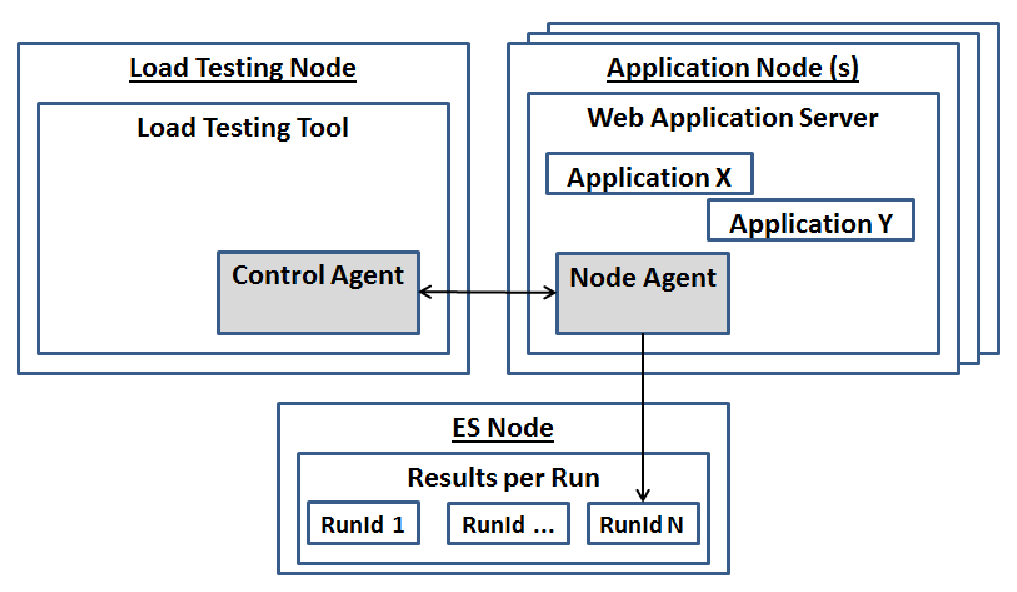
\includegraphics{architecture_dwait}
\caption{High-level Architecture of the solution}
\label{fig_Arch}
\end{figure}

It is important to highlight two assumptions that were considered when defining
the above design. As the scope of this work is the performance testing domain,
it is assumed that a Load Testing tool will always be present in the
testing environment. From the time been, the scope of this work is also focused
on Web Applications (a traditional Java business niche which is also type of 
applications that our industrial partner tests). For this reason, it is also
assumed at this stage that there will always be a Web Application Server in each
one of the application nodes. This assumption has the extra benefit that the
\emph{WAIT Node Agent} is a Web Application. As it uses plain HTTP protocol
to interact with the \emph{WAIT Control Agent}, a single version of \emph{WAIT
Node Agent} could interact with multiples types of \emph{WAIT Control Agent}
(as it is possibly necessary to have one per type of Load Testing Tool) or even
used independently.

Based on the concepts presented here, a prototype has been developed in
conjunction with our industrial partner IBM. The \emph{WAIT Control Agent} was
implemented as a Eclipse Plugin for the Rational Performance Tester (RPT)
\footnote{http://www-03.ibm.com/software/products/us/en/performance},
while the \emph{WAIT Control Agent} was implemented as a Java Web Application,
composed of a single servlet and a few utility classes. Internally, the
application reuses the data gathering scripts that are currently available for
WAIT \footnote{https://wait.ibm.com/#page=dataCollectors}. In both cases,
one of the main reason to chose that technology (Eclipse Plugin and Web
Application) was that they are simple to install, as one of the main drivers of
this work is to reduce the testing effort.

Once installed, WAIT can now be configured as any other resource in RPT. This
scenario is shown in \figurename ~\ref{xxx}. Similarly, once the performance
test has started, WAIT can now be monitored as any other resource in the \emph{Resource View}.
This is shown in the \figurename ~\ref{xxx}. Finally, the WAIT report (which is initially 
created once the first upload is received and then updated after every data
upload) is also accessible within RPT, so that the tester does not need to
leave RPT during the whole duration of the performance test. This is shown
in \figurename ~\ref{xxx}.


%%%%%%%%%%%%%%%%%%%%%%%%%%%%%%%%%%%%%%%%%%%%%%%%%%%%%%%%%%%%%%%%%%%%%%%%%%%%%%%%%%%%%%%%%%%%%%%%%%%%%%%%%%%%
% Experimental Setup / Experiments
%%%%%%%%%%%%%%%%%%%%%%%%%%%%%%%%%%%%%%%%%%%%%%%%%%%%%%%%%%%%%%%%%%%%%%%%%%%%%%%%%%%%%%%%%%%%%%%%%%%%%%%%%%%%

\section{Validation}

This section describes the evaluation of the proposed approach. First the
methodology, metrics and the main threats to validity are
presented. Then, the results of the experiments are presented.

\subsection{Methodology}

<<
Experimental Setup: Application Set. During the experimentation, three real world applications
were used:
- A
- B
>>

4.	METHODOLOGY

<<
We define the following two research questions: Q1 ... Q2 ...
Results of the Experiments: Figure 12 shows the results of the experiments. We answer Q1 with Yes ...
>>

<<
In this section we evaluate our approach. We compare how our approach performs,
(a) when the computation of input data is replaced by the use of random
values, and (b) when the Event Flow Graph is not considered for event sequence
generation.
>>

Phase 1:
o	Objective: Validate WAIT Overhead vs. WAIT-RPT one.
o	Combinations (3):
	WAIT Presence (3): 
	Test without WAIT, 
	Test with WAIT (manual test), 
	Test with WAIT-RPT
	Web-Applications (1): 
	Portal (single node)
	Test configurations*:
	Workloads (1): To be defined (It should be big!) - 2,000
	Duration: 1 hour
	WAIT-RPT configuration:
	HD Threshold: Disabled (so that only the time threshold controls the process).
	Time Threshold: 10 minutes (Constant, so that 6 intervals occur).
	Sampling frequency: 8 minutes.* ----> 30 secs?
* For each identified combination, there will be 3 runs (~9 hours of total execution). WebAppServer restarted before every run.
NOTE: These configurations will be based on expert judgment of the SVT team (reflect “common” practice in the industry?)
Phase 2: 
o	Objective: Validate Architecture (qualitative, quantitative)
o	Combinations:
	WAIT Presence (2):
	Test run without WAIT,
	Test run with WAIT-RPT Integration
	Web Applications (1):
	Either Lotus Connection or JPetStore.
	Test configurations*:
	Workloads (1): To be defined (Tentatively 1, which should be big!) ~2,000 per node (~4,000 assuming 2 nodes)
	Duration: 24 hour (SVT uses 1 hr, 24 hour, 5 days, discarding 1 hr due to relevance and 5 days to do time constraints).
	WAIT-RPT configuration*:
	HD Threshold: 100 MB (pending to confirm).
	Time Threshold: 10 minutes (pending to confirm).
	Sampling frequency: 8 minutes.

For each identified combination, there will be 3 runs (~6 days of total execution). WebAppServer restarted before every run.
NOTE: These configurations will be based on expert judgment of the SVT team (reflect “common” practice in the industry?)
It might also help to show that the reliability of the solution (I might take a look to other “fancy” NFR-related words)

[PENDING: To create figure showing the environment - single PID, then
multi-PID-]

To understand the costs of using WAIT in a distributed environment for long periods of time.
 It will allow defining an initial benchmark of WAIT overheads:
 Impact in throughput of monitored system.
 WAIT usage resource requirements (i.e. HD).
 It can also help to identify additional opportunity areas.

Phase 3: 
Use case … detection benefits of 1 report vs. many! … For the sake of progress, probably the last piece of the experiment!
Injecting defects, showing how they are better/more easily identified. PetStore.
Two dimensions:
- Time: Early detection or trends (stress early detection).
o	Nodes: Environmental issues.

Benefits of WAIT:
- Injecting bugs in JPetStore (Ideas from WAIT + SVT team).
- Benefit of single WAIT report, possible two dimensions:
- Time: Early detection (avoid wasting resources if serious issues identified).
- Nodes: Environmental issues (very likely cause of having an issue in some nodes and other not).
- Meeting to know the fixing side of the performance testing/analysis to get better insights about which use case would be preferrable.
- TEST METRICS: TESTER PRODUCTIVITY? (single case, but give an idea of the benefit)
http://www.softwaretestinggenius.com/articalDetails?qry=967

<<
The teams used performance and load testing tools like
LoadRunner [16] and IBM Rational Performance Tester [15]. They executed reliability runs 
(the ability of a system or component to perform its required functions under stated 
conditions for a specified period of time [24], usually 5 or 7 days) and performance runs 
(short period runs in order to measure something specific, like the response rate [25]).
 As The main aim of both performance and reliability testing
was to ensure that the applications had good performance (transaction and page response rates) even under heavy load, made reasonable usage of memory and didn’t have any memory leaks [31]. The performance of a software system has been described as an indicator of how well the system meets its requirements for timeliness [32]. Smith and Williams [32] describe timeliness as being measured in either response time or throughput, where response time is defined as the time required to respond to a request and throughput is defined as the number of requests that can be processed in some specific time interval. For

15: IBM. Rational Performance Tester. http://www-01.ibm.com/software/awdtools/tester/performance/ 
24: Wikipedia. Reliability engineering.
%http://en.wikipedia.org/wiki/Reliability_%28engineering%29
25: B.Subraya. Integrated Approach to Web Performance Testing: A Practitioner's Guide. IRM Press 2006

By the above case study we tried to see if our approach in
the creation of an expert tool in the field of garbage collection was successful. The measures of success were the ability to
identify bugs and problems that affect the applications as well as additional
test coverage by identifying new types of issues (e.g. finalizers, system.gc, etc). Moreover, the tool should allow a wider range of testers to perform the expert analysis, offering at the same time significant time savings for the expert users. 

The results from using the tool were very encouraging as
many bugs were identified as well as the time saved by using GcLite in some cases was 
quite high. In the table 2, we can see a summary of our case study. We can notice that 
the time saved per application is around 1.6 hours. GcLite’s automated collection and 
analysis of the GC logs, the ease of use, the layout of the output and the use of 
recommendations are responsible for the time savings. We also notice that an average of 
6.5 defects was identified using the tool.

Another important advantage of using the GcLite tool was
the ability to open precise bugs. Testers used the contextual information from the tool 
in order to investigate deeper the issues and provide detailed description in the SPRs 
that they were opening. Furthermore, less experienced testers used this information in 
order to gain a deeper understanding of several re-occurring issues.

In conclusion, the test case showed that the use of an expert
tool that uses the 4 step approach can have several advantages. The time saving from 
using GcLite automated collection of GC logs and analysis instead of another tool in 
some cases was quite high. This was also enhanced by the tool’s ease of use and the 
output’s ease to navigate. Moreover, the amount and variety of bugs that were identified 
shows that GcLite can analyze and discover issues within a GC log by using the 
recommendationEngine. 
>>

3.	KEY METRICS
- Qualitative vs. Quantitative results!
- Qualitative: Possible verbiage about how the detected adoption barriers are
addressed.
- Previously you would have ended with:
- X reports, assuming you monitored X nodes and generated all the reports after
the test execution finished.
- X*Y reports, assuming you monitored X nodes and generated the reports every
1/Y time.
- Now, in both cases you would have ended with a single report.
- Sanity checks: Not lost zip files, hard disk threshold respected.
- Quantitative: Overhead costs: (possible min, max, avg)
- Performance Testing: Response Time, Throughput
- Node Resource Usage: RAM, CPU

A determining factor for performance is that resources have a limited capacity,
so they can potentially halt/delay the execution of competing users by denying
permission to proceed. Quantifying such effects is an important task of SPE.

•	Performance Testing Process

In this paper, when we speak of software performance
testing, we will mean all of the activities involved in the
evaluation of how the system can be expected to perform in
the field. This is considered from a user's perspective and is
typically assessed in terms of throughput, stimulus response
time, or some combination of the two.

Z. THREADS TO VALIDITY:

•	Big variance in 24-hour runs … it seems to different behaviours: Week and
Weekend! (more runs). Environmental issues

<<
- Of course, the results observed cannot be generalised to other applications
different from the two case studies considered here. The presented case studies
are just meant to illustrate the differences that may arise. Wider experiments
need to be executed to get more general conclusions.

Threats to Validity: The main threat to the validity of these results is the fact that only 
three test subjects were used during the experimentation. Despite these subjects being
real world applications being diverse in both the size of the application (lines of
code) and size of the test suite, the limited number of subjects implies that not
all types of system’s are tested. This means that a system with characteristics
that are completly different might present different results.
Another threat is that the number of injected bugs is not enough to lead to
accurate results, as these bugs might simply be “lucky bugs” that intercept a
collar variable.
Naturally, there are also threats that are based on the implementation of the
invariants, the instrumentation or the pattern detector algorithms themselves.
The reduce these threats, additional testing was made prior to the experimentation
to guarantee the quality of the experimental results in this regard.

Threats to Validity: Beyond the selection bias due to the limited availability of open source 
C\# applications, we report one threat to external validity: We evaluated four
C\# open source applications which incorporate the Windows Forms toolkit for
building the GUI. Alternative programming languages and GUI toolkits, e.g., Java Swing,
follow different paradigms of building graphical user interfaces. For example, it
might be not possible to obtain event handlers during the construction of the
EFG. Thus, the construction of the EFG, the generation of parameterized GUI
tests, and the symbolic execution must be adapted to the corresponding environment.
In principle, there is no reason to believe that our approach is not
applicable to other environments.

>>

Statistic references:
Enable Add-on in Excel: http://click4biology.info/c4b/1/2007.htm
%Example in excel, pair t-test:
% http://www.stattutorials.com/EXCEL/EXCEL_TTEST2.html T-Distribution calculations in excel: https://courses.washington.edu/dphs568/course/excel-t.htm
Finding t critical value in excel: http://math.stackexchange.com/questions/10992/finding-critical-value-using-t-distribution-in-excel
how to use t-test in excel (example 2): http://blog.excelmasterseries.com/2010/08/how-to-use-t-test-in-excel-to-find-out.html
Other T-test reference: http://www.ruf.rice.edu/~bioslabs/tools/stats/ttest.html
Excel t-test function: http://www.excelfunctions.net/Excel-Ttest-Function.html
T-test Excel Help: http://office.microsoft.com/en-001/excel-help/ttest-HP005209325.aspx
Good example to learn T-test: http://www.aspfree.com/c/a/braindump/comparing-data-sets-using-statistical-analysis-in-excel/
---
%T-Test description: http://en.wikipedia.org/wiki/Student%27s_t-test
%Null Hypothesis description: http://en.wikipedia.org/wiki/Null_hypothesis
%Student T-Distribution description:
% http://en.wikipedia.org/wiki/Student%27s_t-distribution

Experimental Environment

We installed the benchmark in the system environment depicted in Figure 6. The
benchmark application is deployed in an Oracle WebLogic Server (WLS) 10.3.3 cluster of up to eight 
physical nodes. Each WLS instance runs on a 2-core Intel CPU with OpenSuse 11.1. As a database 
server (DBS), we used Oracle Database 11g, running on a Dell PowerEdge R904 with four 6-core AMD 
CPUs, 128 GB of main memory, and 8x146 GB SAS disk drives. The benchmark driver master, multiple 
driver agents, the supplier emulator and the DNS load balancer were running on separate 
virtualized blade servers. The machines are connected by a 1 GBit LAN, the DBS is connected with 
4 x 1 GBit ports.

%%%%%%%%%%%%%%%%%%%%%%%%%%%%%%%%%%%%%%%%%%%%%%%%%%%%%%%%%%%%%%%%%%%%%%%%%%%%%%%%%%%%%%%%%%%%%%%%%%%%%%%%%%%%
% Section 5: Experimental Results
%%%%%%%%%%%%%%%%%%%%%%%%%%%%%%%%%%%%%%%%%%%%%%%%%%%%%%%%%%%%%%%%%%%%%%%%%%%%%%%%%%%%%%%%%%%%%%%%%%%%%%%%%%%%

\section{Experimental Results}


%[[PENDING: To append results\! (draft_paper_NEW and excel file) should include
%some tables, maybe a graphic or some type]]

1.	[PHASE 1]
o	Compare response time \& throughput with and without WAIT/WAIT-RPT.
o	Compare resource consumption per node with and without WAIT/WAIT-RPT.
+ Testing/Process metrics.
2.	[PHASE 2]
o	Compare response time \& throughput with and without WAIT-RPT.
o	Compare resource consumption per node with and without WAIT-RPT.
o	Validate that there was not “information lost” between the collection and uploading.

3.[PHASE 3]
X,Y to an actual number (use case) … more qualitative, but showing how it is best 1 than many!
Injecting 4 bugs, then run it using the same config than Phase 2 (2 in both nodes, 2 only on a specific one). Then two iterations will be run: 1st to catch up as many issues as possible. The 2nd one to see results after fixing issues (possible an intermediate run might be needed, as some issues might mask other ones) After each run, the detected bugs will be “fixed”.

Benefits: Less Time (setup, monitor, analysis, go/no-go decision) -> Less
Learning curve / Less Error-Prone, Share knowledge / experience (remain), “Real-time”, Keep as light-weight as possible (minimum add-ons + low overhead)

Time-consuming/complex data gathering (one data source per monitored process).
Time-consuming/Complex report analysis (one report per monitored process).
Plus required synchronization with the performance testing execution.
SME expertise required to interpret the reports:
Problem with consumability in parts of Dev, SVT, Perf and Support (few engineers outside of Watson are thread dump experts)

Important to rephrase it as estimated tester time benefit? (at least a high
level estimate … do not forget the time dimension!)

 <<
- (automation) This section presents a case study adapted from [8] and initially discussed 
in [3]. The SUT is a burglar alarm system whose goal is to monitor sensors to detect
the presence of intruders in a building. Consider a test case, presented in [3],
that covers the occurrence of an interruption (transfer to the backup power)
followed by the detection of an intruder finishing with a call to the police. The
objective of the case study presented in this paper is to show how to use the
developed API in test case automation (from step 2 to step 4 in Fig. 1). For this,
a version of the burglar alarm system was developed to run on the FreeRTOS
environment based on industrial PC (x86) port.

- This section summarizes a simplistic case study whose purpose is to illustrate
through a practical example the application of the principles described in Section 3. It
is worthy mentioning that rates have been included as constants declared using
reference values which are not shown. The actual values for these constants should be
changed as more detailed reliability data is available and has no influence on the
scope of this paper.

Empirical Results: In this section the experimental setup is presented, along with the workflow of
the experiments themselves. After that the experimental results are discussed.

>>



%%%%%%%%%%%%%%%%%%%%%%%%%%%%%%%%%%%%%%%%%%%%%%%%%%%%%%%%%%%%%%%%%%%%%%%%%%%%%%%%%%%%%%%%%%%%%%%%%%%%%%%%%%%%
% Section 7: Conclusions
%%%%%%%%%%%%%%%%%%%%%%%%%%%%%%%%%%%%%%%%%%%%%%%%%%%%%%%%%%%%%%%%%%%%%%%%%%%%%%%%%%%%%%%%%%%%%%%%%%%%%%%%%%%%

\section{Conclusions and Future Work}

The identification of performance problems and the diagnosis of their root
causes are very complex and time-consuming activities in highly distributed
environments, which also tend to rely on the expertise of the involved
engineers. The objective of this work was to address the limitations that
prevent the usage of WAIT in the performance testing domain, so that WAIT can be
effective used to reduce the expertise and overall effort required to do
good performance analysis and to identify the root causes of those issues.
To achieve this goal the paper presented a novel automation approach and its
validation, composed of the implementation of a prototype and a study
case with two real-life applications. The results are encouraging as they have
proved that the approach addresses effectively the adoption barriers for WAIT in 
a distributed performance testing environment: The solution has proven being
light-weight, generating a low overhead ([PENDING]). Moreover, from a tester
usability perspective, there are also tangible time savings in terms of the
effort required to detect performance issues.

Future work will concentrate on assessing the practicability of the
approach and its benefits in a major scale through broader study cases with our
industrial partner IBM. It will also be evaluated how best to exploit the
additional functional information that can now be obtained from a tested environment
(i.e. test workload, response time, throughput and transactions) in order to
improve the qualitative and quantitative capabilities of the idle-time
analysis methodology (over which WAIT is based on) to identify more
types of performance problems.

%%%%%%%%%%%%%%%%%%%%%%%%%%%%%%%%%%%%%%%%%%%%%%%%%%%%%%%%%%%%%%%%%%%%%%%%%%%%%%%%%%%%%%%%%%%%%%%%%%%%%%%%%%%%
% Section 8: Acknowledgements
%%%%%%%%%%%%%%%%%%%%%%%%%%%%%%%%%%%%%%%%%%%%%%%%%%%%%%%%%%%%%%%%%%%%%%%%%%%%%%%%%%%%%%%%%%%%%%%%%%%%%%%%%%%%

\section*{Acknowledgments}

We would like to thanks Amar [PENDING], from SVT IBM Dublin, as his expertise
and experience in performance testing helped us through the scope definition and validation of this work.

This work was supported, in part, by Science Foundation Ireland grant 10/CE/I1855 to Lero - the Irish Software Engineering Research Centre (www.lero.ie).

\bibliographystyle{splncs}

\bibliography{dwait_manual,dwait}
%\section*{Appendix: Springer-Author Discount}

\end{document}

Possible footnotes:
•Windows Performance Metrics: http://technet.microsoft.com/en-us/library/cc768048.aspx
•RPT: http://publib.boulder.ibm.com/infocenter/rpthelp/v8r2m1/index.jsp
•iBatis PetStore: http://sourceforge.net/projects/ibatisjpetstore/
• Links about common performance issues:
1. https://onyx.koli.ch/get/6448/3+-+Common+Web+Application+Errors.pdf
2. http://www.crn.com/slide-shows/cloud/231000374/10-most-common-causes-of-web-mobile-app-performance-issues.htm?pgno=1
3. www.tracelytics.com/blog/two-most-common-performance-mistakes/
4. http://gettingreal.37signals.com/toc.php
5. http://jonathanhui.com/top-j2ee-application-performance-problems

PENDING TO:
+ architecture!(proposed approach)
http://blog.optimyth.com/2011/12/should-you-care-about-software-quality-in-these-times-of-economic-crisis


 ----------------------
 
 Related Work - First Draft / Ideas

Automated Performance Testing (support tools).
•	Performance Analysis Tools/Techniques (from WAIT papers).
•	WAIT

<<
(Intro) Related Techniques: In the software development process, performance testing is 
commonly conducted to determine an application's performance as experienced by the user.
In this context, the focus is generally not on a single application session but
on the application in its entirety, i.e., one does not test a single, isolated re-
quest of a single user but rather the performance when many users interact with
the application simultaneously. Software testers commonly use techniques such
as load testing, stress testing, etc., to perform these kinds of tests [3]. There
is a variety of commercial products and free open-source tools available for the
task. For example, IBM's Rational Performance Tester [4] and HPs LoadRunner
[5] both do scalability testing by generating a real work load on the application.
Open-source tools such as Apache's JMeter [6] and Grinder [7] provide a similar
functionality.
Motivated by the large cost for commercial performance testing tools, Chen
et al. created Yet Another Performance Testing Framework [8]. It enables users
to create custom test programs which dene the business operations to be per-
formed during the test. Chen's framework then executes these tasks concurrently.
In [9], Zhang et al. present a cloud-based approach to performance testing of web
services. Their system provides a frontend in which users can specify test cases
which are then dispatched to Amazon EC2 [10] cloud instances for execution.
Similar to all the previous tools, their system is testing the performance under
concurrent user access to the system.
[[
3. Molyneaux, I.: The Art of Application Performance Testing. Volume 1. O'Reilly
Media (2009)
4. IBM: Rational Performance Tester. http://www-01.ibm.com/software/
awdtools/tester/performance/
5. Hewlett Packard: HP LoadRunner. http://www8.hp.com/us/en/software/
software-product.html?compURI=tcm:245-935779
6. Apache Software Foundation: Apache JMeter. http://jmeter.apache.org/
7. Aston, P.: The Grinder, a Java Load Testing Framework. http://grinder.
sourceforge.net/
8. Chen, S., Moreland, D., Nepal, S., Zic, J.: Yet Another Performance Testing
Framework. In: Australian Conference on Software Engineering (ASWEC). (2008)
170 \{179
9. Zhang, L., Chen, Y., Tang, F., Ao, X.: Design and Implementation of Cloud-based
Performance Testing System for Web Services. In: Conference on Communications
and Networking in China (CHINACOM). (2011) 875 \{880
10. Amazon Web Services LLC: Amazon Elastic Compute Cloud (Amazon EC2).
http://aws.amazon.com/ec2/ (2012)
]]

Related Work: The idea of replaying a test execution in a simulator is, of course, not new. The
overall approach is frequently referred to as the capture and replay paradigm,
and has long been studied in different contexts such as testing of concurrent
programs [2]. ... To our best knowledge, our approach is the first to combine replay with model-based
methods for error detection within a test-case generator. Our contribution is not
a theoretical one, but comes from an industrial perspective.

Related Work: Unlike these approaches, our work aims at proposing a generic and platform
independent test system based on the TTCN-3 standard to execute runtime
tests. The proposed test system supports different test isolation mechanisms in
order to support testing different kinds of components: test sensitive, test aware
or even non testable components. Such test system has an important impact on
reducing the risk of interference between test behaviors and business behaviors
as well as avoiding overheads and burdens.

SPE, The commonest approach is purely measurement-based; it
applies testing, diagnosis and tuning late in the development cycle, 
when the system under development can be run and measured (see, e.g.
[2][4][8][9]).

[2] M. Arlitt, D. Krishnamurthy, J. Rolia, “Characterizing
the Scalability of a Large Web-based Shopping System'',
ACM Trans. on Internet Technology, v 1, 2001, pp. 44-69.

[4] A. Avritzer, J. Kondek, D. Liu, and E. J. Weyuker,
"Software performance testing based on workload
characterization," in Proc. WOSP’2002, Rome, , pp. 17-24.

[8] S. Barber, “Creating Effective Load Models for
Performance Testing with Incomplete Empirical Data”, in
Proc. 6th IEEE Int. Workshop on Web Site Evolution, 2004,
pp. 51-59.
[9] S. Barber, “Beyond performance testing”, parts 1-14,
IBM DeveloperWorks, Rational Technical Library, 2004,
www-128.ibm.com/developerworks/rational/library/4169.html

Performance testing on part or all of system, under
normal loads and stress loads [8]. The use of test data
to solve problems is the subject of [9]. This activity is
discussed in Section 3 below.

[8] S. Barber, “Creating Effective Load Models for
Performance Testing with Incomplete Empirical Data”, in
Proc. 6th IEEE Int. Workshop on Web Site Evolution, 2004,
pp. 51-59.
[9] S. Barber, “Beyond performance testing”, parts 1-14,
IBM DeveloperWorks, Rational Technical Library, 2004,
www-128.ibm.com/developerworks/rational/library/4169.html

Technical developments -> Visualization and diagnostics
Understanding the source of performance limitations is a search process, which
depends on patterns and relationships in performance data, often revealed by
visualizations. Promising areas for the future include better visualizations,
deep catalogues of performance-related patterns of behaviour and structure, and
algorithms for automated search and diagnosis.
Present visualization approaches use generic data exploration views such as
Kiviat graphs (e.g. in Paradyn [47]), traffic intensity patterns overlaid on
physical structure maps [47], CPU loading overlaid on scenarios, and breakdowns
of delay [66]. Innovative views are possible. For example, in [60] all kinds of
resources (not just the CPU) are monitored, with tools to group resources and
focus the view. The challenge for the future is to visualize the causal interaction of
behaviour and resources, rather than to focus on just one or the other.
[[
[47] Merson, P. and Hissam, S. “Predictability by construction” Posters of
OOPSLA 2005, pp 134-135, San Diego, ACM Press, Oct. 2005.
[60] J.A. Rolia, L. Cherkasova, R. Friedrich, “Performance Engineering for EA
Systems in Next Generation Data Centres”, Proc. 6th Int. Workshop on Software and Performance, Buenos Aires, Feb. 2007.
[66] C.U. Smith, L. G. Williams, Performance Solutions, Addison-Wesley, 2002
]]

Technical developments -> Bottleneck identification

a search for a saturated resource which limits the system, is a frequent
operation. In [21], Franks et al describe a search strategy over a model, guided by its structure and
results, and detects under-provisioned resource pools and over-long holding
times. It combines properties of resources and behaviour, for a “nested” use of
resources. It scales to high complexity, is capable of partial automation, and
could be adapted to interpret measured data. A multistep performance enhancement
study using these principles is described in [83].
Another search strategy purely over data ([9], part 7) focuses on reproducing
and simplifying the conditions in which the problem is observed. The actual diagnosis
of the cause (e.g. a memory leak) depends on designer expertise.
A bottleneck search strategy combining the data and the model could detect more
kinds of problems (e.g. both memory leaks and resource problems) and could
provide automated search assistance.
Patterns (or anti-patterns) related to bottlenecks have been described by Smith
and Williams [66] and others (e.g., excessive dynamic allocation, “one-lane bridge”).
For the future, more patterns and more kinds of patterns (on measurements, on
scenarios or traces) will be important. Patterns that combine design, model and
measurement will be more powerful than those based on a single source.
[[
[9] S. Barber, “Beyond performance testing”, parts 1-14, IBM DeveloperWorks,
Rational Technical Library, 2004, www-128.ibm.com/developerworks/rational/library/4169.html

[21] G. Franks, D.C. Petriu, M. Woodside, J. Xu, P. Tregunno, 
“Layered Bottlenecks and Their Mitigation”, Proc 3rd Int. Conf. on Quantitative
Evaluation of Systems, Riverside, CA, Sept. 2006.

[83] J. Xu, M. Woodside, and D.C. Petriu, 
“Performance Analysis of a Software Design using the UML Profile for
Schedulability, Performance and Time”, in Proc. 13th Int.
Conf. Modeling Techniques and Tools for Computer Performance Evaluation, Urbana,
USA, Sept. 2003 ]]

Scalability analysis and improvement is largely a matter of identifying
bottlenecks that emerge as scale is increased, and evolving the architecture. Future
scalability tools will employ advanced bottleneck analysis but will depend more
heavily on models, since they deal with potential systems.


•	Performance Testing Tools? (HP Load Runner, Jmeter, RPT).

[Pending to see where better to fit these points:]
Benefit: Tools usability, productivity increase (less time identifying issues and their root cause), any benefit in the consolidation (other than reducing from N*M reports to 1), i.e. trends in time and/or nodes (probably good input from performance team):
* How does the process currently work? (steps and time) i.e. ~2 hours debugging, 2-4 RCA + fixing OO
* Issues in different nodes sound like environmental ones?
* Issues in different times (kind of trending) might involve the application?
They refer to “end to end” testing … the most common issue are deadlocks.

He uses different tools:
- Heap dumps: WAIT?
- Thread dumps: WAIT (locks, contentions) … around every 5 - 10 mins / ISA (performance analysis kit based on Eclipse).
- Overall development expertise (i.e. architecture, layers, frameworks, tools).
- Code profiling: tprof to profile in real time (recording every 1-2 mins to know the CPU usage per transactions); jprofiling (single transaction costs, such as CPU usage).
- Database: Tunning of SQL queries (or expert systems that encapsulate the identification of the most common issues).
- GC: gclite (expert system) or jmap.

Today, the state of industrial performance measurement and testing techniques is
captured in a series of articles by Scott Barber [8][9] including the problems
of planning, execution, instrumentation and interpretation.

[8] S. Barber, “Creating Effective Load Models for Performance Testing with
Incomplete Empirical Data”, in Proc. 6th IEEE Int. Workshop on Web Site Evolution, 2004,
pp. 51-59.
[9] S. Barber, “Beyond performance testing”, parts 1-14, IBM DeveloperWorks,
Rational Technical Library, 2004, www-128.ibm.com/developerworks/rational/library/4169.html

The tools used by performance analysts range from load generators, for supplying
the workload to a system under test, to monitors, for gathering data as the
system executes.

Key message/conclusion: The identification of the root causes of performance issues, relies very heavy on the expert knowledge of the user + requires a lot of different tools. There is no possible to indicate an average time per issue identification, but overall is very challenging/time-consuming.

 
 ----------------------------
  